%!TEX program = pdflatex
\documentclass{llncs}
\usepackage[T1]{fontenc}
\usepackage[utf8]{inputenc}
% \usepackage{natbib}
\usepackage[version=4]{mhchem}
\usepackage{graphicx}
\usepackage{todonotes}
% \usepackage{wrapfig}
% \usepackage{subfig}


\begin{document}

\pagestyle{plain}
\title{ETDetective}
\subtitle{Estimation of Reaction Constants Triggered by Electron Transfer in Top-Down Mass Spectrometry}
\author{Michał Ciach\inst{1} \and Mateusz Krzysztof Łącki\inst{1} \and Błażej Miasojedow\inst{1} \and Frederik Lermyte\inst{2,3} \and Dirk Valkenborg\inst{3,4} \and Frank Sobott\inst{2,5,6} \and Anna Gambin\inst{1} }

\institute{
        Faculty of Mathematics, Informatics and Mechanics, University of Warsaw, Poland, \and
        Biomolecular and Analytical Mass Spectrometry Group, Dept. of Chemistry, University of Antwerp, Belgium, \and
        Centre for Proteomics, University of Antwerp, Belgium,\and
        Interuniversity Institute for Biostatistics and Statistical Bioinformatics, Hasselt University, Hasselt, Belgium \and
        Astbury Centre for Structural Molecular Biology, University of Leeds, Leeds LS2 9JT, United Kingdom, \and
        School of Molecular and Cellular Biology, University of Leeds, LS2 9JT, United Kingdom.
}

\maketitle
\begin{abstract}
        Electron transfer dissociation (ETD) is a versatile technique used in mass spectrometry for high-throughput characterization of proteins. It consists of several competing reactions triggered by the transfer of electron from its anion source unto the sample cations. Relative quantities of the products of these reactions can be retrieved from mass spectra.

        Here, we study these results from the perspective of the reaction kinetics. A formal mathematical model of the ETD is introduced and parametrized by intensities of the existing reactions. Also, we introduce a method to estimate the reaction intensities by solving a nonlinear optimisation problem. The presented method is proves highly robust to noise on in silico generated data. What is more, our model explains a considerable amount of experimental results gathered under various experimental settings.
\end{abstract}

\section{Introduction}
\textbf{Motivation.}
        Owing to the important role proteins play in various biological processes, as well as the significantly greater complexity of the proteome compared to the genome \cite{Smith2013-km} there is significant need for analytical techniques capable of high-throughput protein characterization. Mass spectrometry (MS) is a highly valuable technology in this context; however, automated methods for (tandem) MS data analysis are somewhat lagging, particularly for top-down (i.e. without enzymatic digestion of proteins before MS analysis) and native (i.e. while preserving noncovalent interactions during sample preparation and in the gas phase) approaches.



        One of the principal fragmentation methods used in top-down mass spectrometry is Electron Transfer Dissociation, ETD, which is based on the interaction of a multiply charged, non-radical protein/peptide cation and a radical reagent anion \cite{Syka2004-rg,Zhurov2013-ua}. However, while this method is becoming ever more ubiquitous in MS-based proteomics analyses, important questions remain regarding the precise reaction mechanism, and which level(s) of protein structure can be probed using ETD \cite{Sohn2009-zv,Sohn2015-rp}. Shedding more light on the nature of ETD can therefore lead to optimization of instrumental settings and to better identification of peptide sequences and post-translational modifications.

        There are several other fragmentation techniques, most importantly the Collision Induced Dissociation, CID, where the cleavage is induced by collisional activation, i.e. bombardment with non-reactive molecules \cite{Mitchell_Wells2005-gn}. A major disadvantage of the CID is that it often leads to loss of posttranslational modifications, particularly phosphorylation \cite{Kim2012-yz}. The Electron Transfer Dissociation has been also found to provide more uniform fragmentation than the CID, which breaks mostly the weakest bonds\cite{Kim2012-yz,Zhurov2013-ua}. However, a notable amount of work has been devoted to analyzing and mathematical modelling of the CID reaction; see, for example, \cite{Zhang2004-fp,Zhang2005-jn,Wysocki2000-am}, while the ETD has received less attention.

\textbf{Electron Transfer Dissociation and side reactions.}
        The fragmentation in ETD is induced by the transfer of an electron from a radical anion to the sample peptide/protein cation and results in a cleavage of one of the peptide bonds, \ce{N-C_\alpha}, of the protein’s backbone. The sample cations get positively charged during the electrospray ionisation (ESI) step, see \cite{Fenn1989-mp}, in which protons are attached to the sample molecules, leading to the formation of \ce{[M + nH]^{n+}} ions, i.e. adding both charge and mass to the analyte molecule M.

        When a cation interacts with an anion, several reactions may occur:

        \begin{enumerate}
                \item In the \textit{default} reaction, ETD, the cation accepts the electron and, after rapid neutralization of charge and a series of electron rearrangements, a backbone \ce{N-C_\alpha} bond breaks leading to the formation of so called \ce{c} and \ce{z} fragment where c-ion contains the N-terminus and z-ion the C-terminus.

                \item the cation accepts the electron but no fragmentation is observed, and the electron stays on the analyte. this is referred to as ETnoD, as no dissociation occurs.

                \item one of the cation’s protons is transferred to the anion; a situation referred to as a proton transfer reaction, or PTR.
        \end{enumerate}


        The above reactions are formalized in Fig.~\ref{img::reactions}.
        \begin{figure}[h]
                \center
                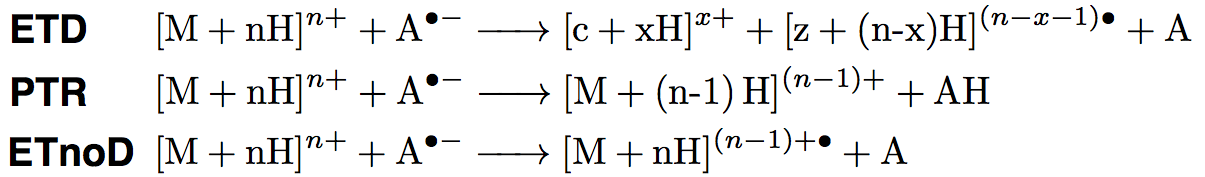
\includegraphics[width=.8\textwidth]{reactions.png}
                \caption{Chemical formulas of presumed ion-ion reactions. During ETD a backbone bond between the \ce{C_\alpha} and N atom is broken, resulting in \ce{c} and \ce{z} ions. During PTR, the anion accepts one of the protons that charged the precursor cation. During ETnoD, the radical is transferred from the anion onto the cation without inducing fragmentation, thereby reducing its charge. Note that the ETnoD product is heavier than the PTR product by one hydrogen mass (as the mass of an electron can be neglected).}\label{img::reactions}
        \end{figure}

        The appearance of the ETnoD fragments in the experimental data can be linked to the folding of proteins: although backbone cleavage occurs, noncovalent interactions keep the resulting fragments from separating, see \cite{Lermyte2014-vu,Lermyte2015-oy} [Lermyte, JASMS, 2014 and Lermyte, Proteomics, 2015]. The ETnoD can also be caused by accommodation of an electron on the backbone of the protein, e.g. in an aromatic side chain. It is assumed that, regardless of the precise reaction mechanism, the electron obtained by ETnoD causes neutralization of an ESI-generated proton, to which we subsequently refer as a quenched proton \cite{Lermyte2015-lm}.

        In all of the reactions described above, the net charge of a protein cation reduces by one. Also, the mass of the radical can be neglected, as most modern instruments do not resolve it. The isotope distributions of PTR and ETnoD products will show considerable overlap, especially for large molecules, as illustrated in Fig.~\ref{img::masstodon}. Cations can undergo several reaction events, being multiply approached by different anions. However, the so-called internal fragments of proteins, i.e. resulting from two backbone cleavage events, are usually not observed suggesting that double ETD scarcely ever occurs. On the other hand, there is a lot of evidence of multiple ETnoD and PTR occurring on one analyte molecule, see \cite{Lermyte2015-li}.

        \begin{figure}[h]
                \center
                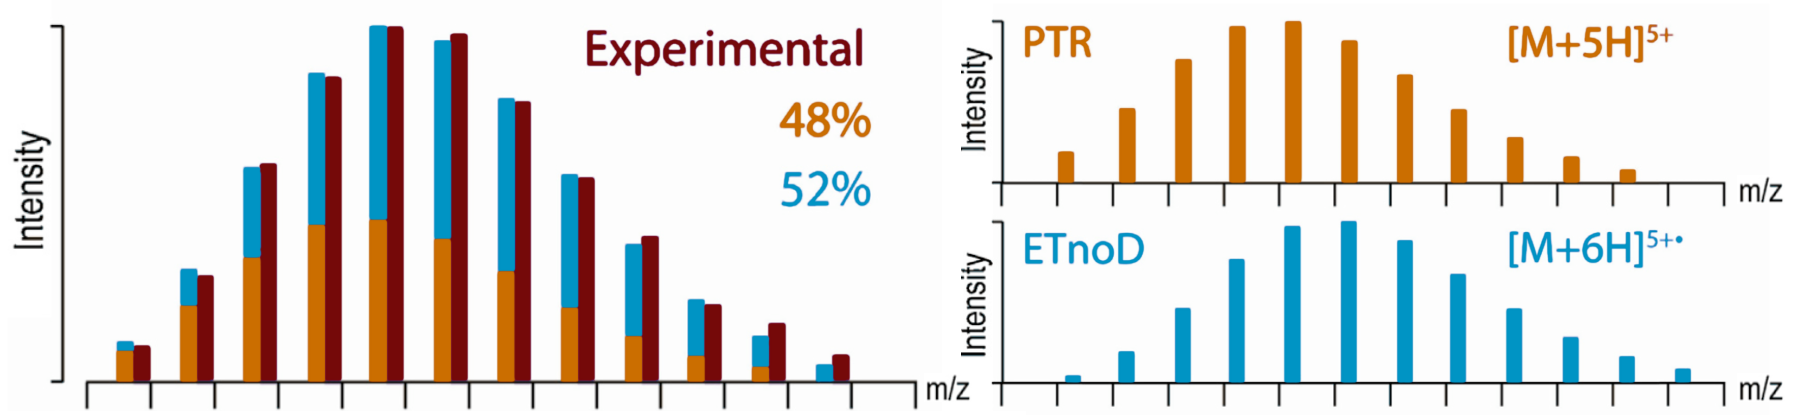
\includegraphics[width=.8\textwidth]{masstodon.png}
                \caption{The deconvolution of an isotope cluster (left) that can be theoretically traced to be a mixture of two overlapping (differing by one hydrogen mass) isotope structures (right) as performed by MassTodon.}\label{img::masstodon}
        \end{figure}

        The peptide bond cleavage induced by ETD is believed to be fairly uniform. A notable exception from this rule is the peptide bond of proline. ue to the ring structure of this amino acid, the \ce{c}- and \ce{z}-ions are held together together after the \ce{N-C\alpha} bond cleavage.  Furthermore,  specific tertiary structure of the protein can also prevent dissociation: the two fragments can simply remain entangled. Experiments show that delivering extra energy to such pairs easily leads to their disentanglement \cite{Lermyte2017-zt}. As a consequence, different fragments may show different intensities of ETnoD, as they vary in their tertiary structure.

        A specific type of \ce{N-C\alpha} bond cleavage occurs on the N-terminus, leading to a loss of one ammonia molecule. The precise mechanism of this reaction is not known. However, the current work we assume this reaction to be an ETD, and the ammonia molecule is treated as a \ce{c} fragment. Therefore, the number of possible ETD cleavage sites is equal to the number of amino acids other than proline in the protein/peptide sequence.

        Only charged ions are observed in the mass spectrometer.

\textbf{Related research.}
        Various approaches have been taken to model electron transfer driven reactions \cite{Breuker2004-az,Simons2010-gy,Zhurov2013-ua,Turecek2013-fq}. A somewhat similar approach to the one taken by us was presented by Zhang \cite{Zhang2004-fp,Zhang2005-jn,Zhang2011-lg}, who uses a kinetic model to study fragmentation. In \cite{Zhang2010-fp}, Zhang adapts the model to explicitly model mass spectra obtained with the use of ETD. The model is complex (having 280 parameters) and relies on assumptions that are backed by theoretical considerations that use many notions of statistical mechanics. The model was fitted to a training dataset consisting of more than 7000 ETD spectra simultaneously.

        On the other end of the possible spectrum of approaches to model protein fragmentation, a notable amount of literature has been built up around the idea of purely data-driven prediction of the intensity of peptides in tandem MS experiments \cite{Elias2004-fr,Arnold2006-wn,Degroeve2013-ej} . A more exploratory approach targeted at studying fragmentation patterns was taken by Li \cite{Li2011-mq}. That said, the above approaches have been applied mainly to study a different type of fragmentation reaction - the Collision Induced Dissociation, which widely differs from the ETD.

\textbf{Our contribution.}
        We propose a formal model of the electron driven reactions occurring inside the mass spectrometer. The modelling strategy we follow was first developed by Gambin \cite{Gambin2010} to study the degradation of proteins induced by the exopeptidase enzyme. A particular feature of this phenomenon is the irreversibility of the process: peptides cannot merge back into bigger compounds. This simple trait leads to a considerable simplifications in the dynamics of the continuous time Markov Jump Process used to model the phenomenon: the average numbers of proteins at a given time can be obtained by solving a system of recursively dependent ordinary differential equations, ODEs.

        Likewise, in the context of ETD, during each reaction the cation loses at least one charge and it is impossible for it to charge itself back; thus, there are no cycles present in the dynamics of this problem. The solution to this problem can be obtained conceptually in the same way: given initial values of parameters describing the intensities of transitions in the process, one can solve the ODEs with a recursive algorithm. The parameters can be optimized to minimize the difference between the calculated averages and the actual experimental data.

        Gambin \cite{Gambin2010} have used LC-MS experiment data. Here, we use mass spectra gathered in controlled experiments, obtained for highly purified compounds. The identity of the precursor ion and all fragments obtained given a set of possible reactions is known and the quantities of these fragments can be established using our in-house developed identification tool called MassTodon \cite{Lermyte2015-lm,Lermyte2017-zt}. Given a mass spectrum, MassTodon outputs a list of reaction products together with their estimated intensities. It merges intensities of peaks that can be traced to originate from different isotopologues of the same molecule and also deconvolves isotope clusters into their sources or origin, see Fig.~\ref{img::masstodon}.

        The obtained information is more compact, but still not easy to interpret: the number of possible fragments is linear in the length of the amino acid sequence, assuming no internal fragments can be observed, and quadratic in the number of charge. The retrievable data can be presented as a point in a highly dimensional space, each coordinate corresponding to a fragment’s sequence, charge and number of electrons gained via ETnoD.

        The method we propose massively reduces this dimensionality. It is natural to assume that the resulting spectra are produced as an outcome of some stochastic chemical process governed by the intensities of possible reactions. A process described by a small number of parameters can be also more easily visualised and thus -- more easily understood. A low-dimensional representation of spectra by a set of easily interpretable parameters considerably simplifies both the comparison of the spectra obtained from the instrument under different experimental settings and the comparison of spectra coming from different instruments.

\textbf{Organisation of the paper.}
        First, we introduce the theoretical considerations behind our model. Then, we describe the procedures used to obtain our datasets, both experimental and  simulational , used to assess the quality of the model. Then, we describe the performance of the model and finally we sketch existing problems and possible extensions for the future work.


\section{Formal model of the ETD reaction}

        Following the ideas outlined in \cite{Gambin2010}, we model the ETD as a continuous time Markov Jump Process, MJP. To describe the state space for our model we introduce the reaction graph, which is a bipartite directed graph with two types of nodes we call molecular species and reactions. In the context of ETD, the molecular species correspond to cations that are substrates or products of the studied reactions: ETD, ETnoD, and PTR, see Fig.~\ref{img::petrinet}. In the current setup, each molecular specie u can be uniquely described by: (1) the sequence of amino acids s, (2) the charge of the cation q, and (3) the number of protons g that have been paired with electrons, so that $u = (s,q,g)$. Remembering how many times this occurred is necessary to correctly calculate the mass of cation.  Additionally, all molecules that cannot be observed - such as analyte molecules that have lost all charged protons - are merged into one molecular specie we call the cemetery. Note that we do not assume to know the precise position of protons along the molecule. Instead, we concentrate on studying the changes in their numbers rather than their precise positioning, with assumption that ESI-generated protons can only be attached to basic amino acids.

\begin{figure}[h]
        \center
        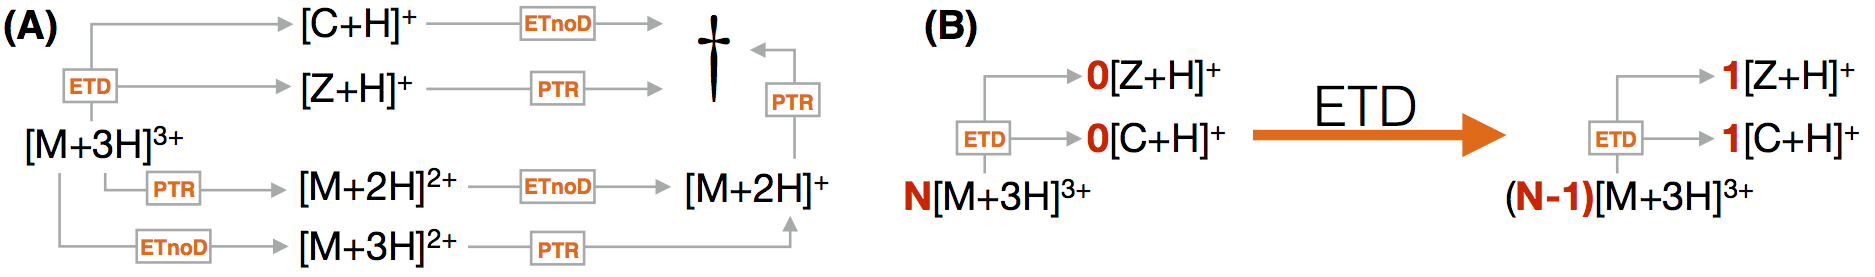
\includegraphics[width=.8\textwidth]{petrinet.png}
        \caption{A simplified Markov Jump Process of the ETD process. The \textit{molecular species} are depicted in black and the \textit{reactions} in orange. The dagger symbolizes the \textit{cemetary} -- a specie that collects all molecules introduced to the instrument that lost their charge during in the cascade of reactions. The reaction graph serves as a board for \textit{tokens}. Counts of tokens are plotted in red in panel (B). During each reaction a token disappears on the substrate side and product tokens appear: one in case of ETnoD and PTR, two in case of ETD, as seen in (B).}\label{img::petrinet}
\end{figure}

        The molecular species are occupied by tokens that represent the numbers of given molecular species. We denote the number of tokens at place $u$ by $x_u$. The state $x$ of the MJP is defined as a collection of all such counts at a given moment in time, so that $x = (x_u)$.  From a state $x$ the system can evolve to another state following one of possible transtions, like in Fig.~\ref{img::petrinet} (B).

        We investigate $L$ fragmenting reactions, where $L$ is equal to the number of amino acids of the protein under study minus the number of prolines that ETD cannot fragment. We also consider two other reactions corresponding to ETnoD and PTR, that change one substrate into one product.

        In the continuous time MJP reactions are drawn from a precise distribution. Another distribution describes when a reaction can happen. Here, time is modelled as an interval ranging from $0$, the beginning of the process, to $1$,  the moment of observation. In such setting, one can investigate how probable is it for the process $X$ to end up in state $x$ at a given time $t$. We denote that probability by $p_x^t$. The derivative of this quantity follows the master equation,
                $$\dot{p}_x^t = \sum_{y\not=x} p_y^t Q_{yx} - p_x^t \sum_{y\not=x} Q_{xy},$$
        Above, $Q_{xy}$ is the intensity of the jump from state $x$ to $y$. The intensity equals $0$ if $y$ cannot be reached from $x$ by means of one reaction $R$. Otherwise, the intensity is assumed to be proportional to the number of the substrate molecules, $Q_{xy}=c_R x_{s_R}$,  where $c_R$ is a constant related only to the type of reaction, described in detail later on.

        The average numbers of cations at that place $u$ is $E_u^t= \sum_x x_up_x^t$. At $t=0$, the process is deterministic: all tokens can be found only in the precursor node with maximal charge state, a place we call the root, $r$. Thus, $E_r^0=N$ and $E_u^0=0$ if $u \not= r$. Later in time, the averages evolve according to
        $$\dot E_u^t=\sum_x x_u \sum_{y\not=x} p_y^t Q_{yx} -\sum_x x_u p_x^t \sum_{y\not=x} Q_{xy}.$$
        The double sums iterate over tuples $(x,y)$ or $(y,x)$ that correspond to reactions that change the first state to another by moving tokens. One can neglect states that cannot be obtained from other states, as then the intensity $Q_{xy}$ equals zero. This, and the asumption on the form of intensity, $Q_{xy}=c_Rx_{s_R}$, leads to
        $$\dot E_u^t = \sum_R cR \left[ \sum_{x:x=Ry}  x_u (x_{s_R}+1) p_{R^{-1}x}^t- \sum_{x} x_u x_{s_R} p_x^t \right].$$
        Above, $Ry$ denotes the state obtained from $y$ after reaction $R$ and $R^{-1}x$ denotes the state that results in $x$ when $R$ happened. For a given $R$,
                $$\sum_{x:x=Ry} x_u (x_{s_R}+1) p_{R^{-1}x}^t = \sum_{y}  (Ry)_u y_{s_R} p_y^t = \sum_x (Rx)_u x_{s_R} p_x^t,$$
        as we can restate the sums in terms of states from before transtion $R$ and retag $y$ for $x$. Thus, $\dot E_u^t = \sum_R c_R \sum_x   \left[(Rx)_u-x_u \right] x_{s_R} p_x^t$. The term $\left[(Rx)_u-x_u\right]$ equals $1$ if place $u$ is a product of reaction $R$, $-1$ for substrate, and $0$ otherwise. Therefore, it is a value dependent on $R$ and not on particular state $x$. Denote it by $K_R$. Then
                $$\dot E_u^t = \sum_R c_R K_R \sum_x x_{s_R} p_x^t = \sum_R c_R K_R E_{s_R}^t = \sum_{R:u\in P_R} c_R E_{s_R}^t - E_u^t \sum_{R: u=s_R}c_R,$$
        where $P_R$ are the products of reaction $R$. The inflow of molecules in place $u$ is proportional to the average numbers of the parent molecules of $u$. Their proportionality constants are equal to reaction intensities. The outflow depends on types of reactions that lead out of this place. In the considered problem, at most one transition can lead from one place to another. We can rewrite the above formula to underline the dependence of the average amount of molecular specie $u$ upon other species $v$ that can be turned to $u$ by some reaction (which we call the parents of $u$)
        $$ \dot E_u^t = \sum_{v\rightarrow u} \lambda_{vu} E_v^t - \lambda_{uu}E_u^t.$$
        The above system of ODEs is recursive and can be solved from the root r downwards. For the root, $\dot E_r^t=-\lambda_{rr} E_r^t$, so that function $E_r^t= Ne^{-\lambda_{rr}t}$ solves it. Say that one computed the solutions for all molecules $v$ that are parents of $u$. The form of the corresponding functions, $E_v^t$, is then known; denote by $f_{>u}$ the sum of these solutions weighted by appropriate lambdas. By definition, the root is a parent of its children $u$, which we denote by $r \geq u$. Thus, $\dot E_u^t=f_{>u}(t)-\lambda_{uu} E_u^t$. Given that $E_u^0=0$ for all $u_r$, the solution to this equation is, by straightforward integration, $E_u^t=e^{-\lambda_{uu}t} \int_0^t e^{\lambda_{uu}s} f_{>u}(s)ds$.
        Consider that $u$ is one of the sons of root $r$: plug in $f_{>u}(s)=E_r^s$ above and perform integration to obtain $E_u^t= \frac{N}{\lambda_{rr}-\lambda_{uu}}(e{-\lambda_{uu}t}-e^{-\lambda_{rr}t})$.
        This holds only when $\lambda_{vv}=\lambda_{uu}$, which is true as shown below.
        Similarly, one can prove that the general solution is $E_u^t=\sum_{v>u}b_{vu}e{-\lambda_{vv}t}-b_{uu}e^{-\lambda_{uu}t}$, where $b_{vu}= \frac{1}{\lambda_{uu}-\lambda_{vv}} \sum_{w: v\geq w \rightarrow u} \lambda_{wu}b_{vw}$ and  $b_{uu}=-\sum_v b_{vu}.$

        Intensities are assumed to factorize  so that $\lambda_u = I q_i^2 P_{R_u}$, where $I$ is the overall intensity of all reactions, $q_u$ is the charge of molecules in place $u$, and $P_{R_u}$ is the probability that reaction $R_u$ happened if given that some reaction occurred. For ETnoD and PTR respectively $P_{R_u}=P_\text{PTR}$ and $P_{R_u}=P_\text{ETnoD}$. The presence of the squared charge is motivated by arguments presented by McLuckey \cite{McLuckey1999-su}.
        The case of ETD is more complex, as it can cleave different bonds. We denote the probability of the cleavage of the $l^\text{th}$ bond by $P_{\text{ETD}_l}$. Additionally, one has to divide the $q-1$ protons and $g$ quenched protons between both the \ce{c} and \ce{z} fragments, so that $q_c+q_z=q-1$ and $g_c+g_z = g$. In its turn, the division of remaining $q-1$ protons and $g$ quenched protons depends on the available number of basic amino-acids on both fragments, denoted by $B_c$ and $B_z$. It occurs with probability $P_l(q_c, g_c) = \frac{ \binom{B_c}{q_c}\binom{B_z}{q_z} }{ \binom{B_c+B_z}{q-1} } \frac{ \binom{B_c - q_c}{g_c} \binom{B_z-q_z}{g_z} }{ \binom{B_c+B_z-q+1}{g} }$,
        which corresponds to placing the $q_c$ charged (i.e. non-quenched) protons out of $q$ charged protons of the substrate molecule on the basic sites of the fragment peptide, followed by placing $g_c$ quenched protons on the remaining free basic sites. The probability does not depend upon the order of this procedure (i.e. placing quenched protons after charged ones or the other way around). Also, summing $P_l(q_c, g_c)$ over all possible placements, i.e. $(q_c, g_c)$ pairs, results in $1$. To conclude, the probability of the ETD on the $l^\text{th}$ amino acid with a given proton distribution among fragments equals $P_{R_u}=P_{\text{ETD}_l} P_l(q_c, g_c)$. The probability of observing any ETD reaction, $P_\text{ETD}$, can be obtained by summing $P_{\text{ETD}_l}$ over possible cleavage sites.

        Overall, the model is parametrized by the total reaction intensity $I$, two reaction probabilities $(P_\text{PTR}, P_\text{ETnoD})$ and $L$ ETD reaction probabilities $P_\text{ETD}$. For a given vector of model parameters  we can obtain the average number of cations for each molecular specie at time $t=1$, $e_u^1 =e_{u\theta}$. On the other hand, using MassTodon we obtain the estimates $y_u$ of the percentual content of that molecular specie in the experimental mass spectrum. For a given $\theta$, we measure the error using a logarithm of a sum of squared errors, $d(e_\theta,y) = \log \sum_u (e_{u\theta}-y_u)^2$. The element $\theta^*$ that minimizes the error is our estimate of the true value of the parameters.


\section{Materials and Methods}

        \textbf{Simulations.} Numerical simulations of ETD reaction were performed to assess the quality of the fitting procedure in fully controlled conditions. The simulation was performed as follows: we start with a given number $N$ of substance P precursor cations. We simulate the electrospray ionization by placing a given number of protons on randomly chosen basic amino acids. Then, we simulate the Markov Jump Process using standard simulation techniques \cite{Gillespie1977-fr}, noting that our process can be simulated as if the cations reacted independently of each other. Ions that find themselves in the same state at the end of the simulation are aggregated. The resulting counts of ions simulate results obtainable with the MassTodon software.

        We also analyze the robustness of the fitting procedure to noisy or missing data. The random noise is modelled by adding gaussian noise to the counts, with zero mean and standard deviation expressed as a given percentage of the count. Missing data is modelled by randomly removing a given proportion of the peaks. Finally, the counts obtained in this way are normalized to one. Altogether, the simulation was repeated $100$ times for $29$ different values of data distortion parameters, see Fig.\ref{fig::kokos}.\todo{Change that figure.}

        \begin{figure}[h]
                \center
                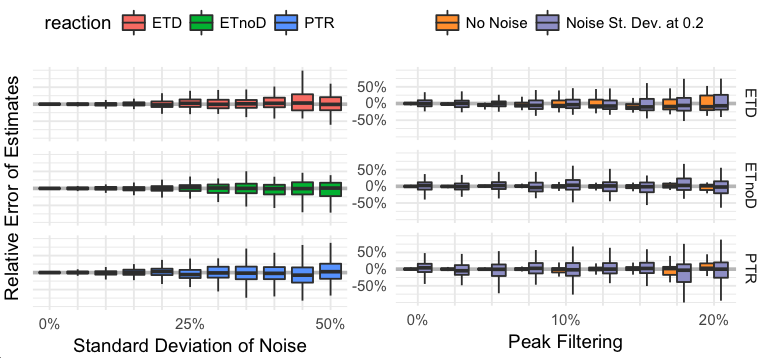
\includegraphics[width=.8\textwidth]{kokos.png}
                \caption{ Relative errors of the fitting procedure on in silico Substance P data. The known true values of parameters are respectively $P_\text{ETD}=30\%, P_\text{ETnoD}= 25\%, P_{PTR}= 45\%$. Cleavage probabilies were assumed to be uniform. Each boxplot summarizes the results of $100$ independent simulations. The left panel presents the response of the relative error of the estimates to the increasing amount of noise in the intensities reported by MassTodon. In that case, we did not additionally model missing data (by filtering peaks). On the right panel, we study the impact of random removal of peaks, both in noiseless conditions (in gold) and with a modest amount of noise (standard deviation set to $20\%$ of the intensity of the simulated molecule).
                }\label{fig::kokos}
        \end{figure}


        \textbf{Experimental data.} Substance P (Sigma S6883, 1.4 kDa) was dissolved at a concentration of 4 $\mu$M in water/acetonitrile v/v 50/50 and 1\% formic acid added. Approximately 5 $\mu$L of this solution was transferred to a gold-coated glass capillary prepared in-house and infused into the Synapt G2 mass spectrometer (Waters, Wilmslow, UK) using the nanoflow version of the Z-spray ion source, with a capillary voltage of 1.2 – 1.6 kV, minimal (<0.2 bar) nanoflow gas pressure, a backing pressure of 2.4 mbar and a source pressure of 1.6e-3 mbar. In ETD mode, reagent (1,4-dicyanobenzene) vapor is carried by a nitrogen flow at room temperature to the glow discharge needle located between the sampling cone and extraction cone, where radical anions are generated. The polarity of the ion optics up to and including the entrance of the trap cell is continuously switched, and after filling the T-wave trap cell with ETD reagent for 0.1 s, it is trapped there and allowed to interact for 1.0 s with the nano-ESI generated analyte cations, before the cycle starts again. Cation precursors and reaction products are axially propelled through the ETD reagent ‘‘cloud’’ in the trap cell by means of a travelling wave, the amplitude (‘height’) and velocity of which determine the extent and time of ion–ion interaction. The glow discharge was tuned to provide a signal of approximately 2e6 reagent counts per second (make-up gas flow 35 mL/min, discharge current 20 $\mu$A). Instrument settings were as follows: sampling cone 60 V, extraction cone 2 V, trap pressure 6.2e-2 mbar, trap collision energy 4 V, trap DC bias 8 V, transfer pressure 1.2e-2 mbar. The instrument was operated in Sensitivity mode and fitted with a 32 K quadrupole. For relative peak intensity measurements, the spectrum was smoothed (2x three-channel Savitsky-Golay method) and centered using MassLynx (version 4.1).
%
        \section{Results}
        We have tested the model and the fitting procedure on both simulated and experimental data to assess their robustness and to estimate real reaction intensities.
%
        \textbf{In silico.} The model has been fitted to in silico data obtained as described in the Materials and Methods section. The fitting procedure turned out to be fairly robust against moderate noise (up to $ \approx 50\%$ of the signal intensity) and missing data, see Fig.~\ref{fig::kokos}. As can be seen, the results of the fitting procedure are unbiased in most conditions, being off only when we trim nearly $50\%$ of the input data. Confronted with large losses of data (more than $30\%$), the procedure breaks down and the procedure overestimates the amount of the ETD fragmentation. Note that in these cases, estimates obtained for ETnoD are very different when modelled with and without additional noise. On noiseless data and data with moderate amount of noise (up to $50\%$ of variation in simulated intensities), the model was able to predict the reaction intensities with very high accuracy (relative errors rarely surpass $10\%$). Generally, the obtained estimates were unbiased, with low variance.

        \textbf{Fitting to experimental data.} The model has been fitted to $53$ Substance P spectra, obtained at various travelling-wave height/velocity combinations as described in the Materials and Methods section. After fitting the model to the data, the validity of the model was further investigated by computing the percentage of the experimental spectrum explained by the theoretically predicted spectrum. We call this value the Explanation Percentage (EP) and define it to be the common part of a theoretical and experimental spectrum. Since both spectra are normalized so that they sum to one, the Explanation Percentage can be expressed in a simple formula,
        $$ EP = \sum_u \min\{y_u, e_u^\text{norm}\}.$$

        Note, that because of normalization, $0 \leq EP \leq 1$. We present the Explanation Percentage calculated for considered data sets in Fig.~\ref{fig::melon} (two panels in the upper left corner): the typical values are between $73\%$ and $98\%$. These results are very promising given that the assumption that process intensities are constant, is rather strict, as discussed later on.

        \begin{figure}[h]
                \center
                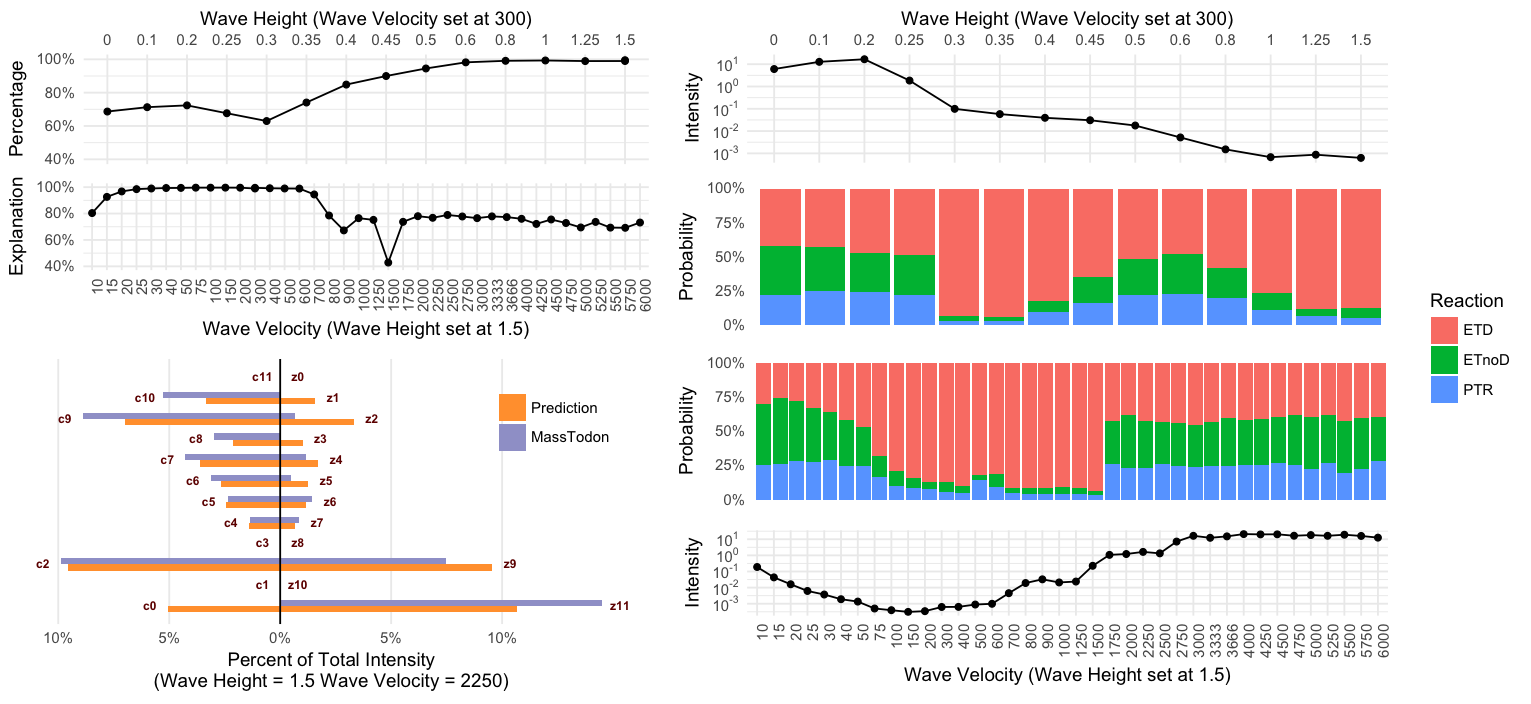
\includegraphics[width=.8\textwidth]{melon.png}
                \caption{ Results of fitting to experimental data preprocessed by the MassTodon software. Two black-and-white plots in the top left corner report the Explanation Percentages calculated for the input data. Below, we present results of fitting the model to the fragments obtained at Wave Height $= 1.5$ and Wave Velocity $= 2250$. Intensities of the \ce{c} fragments are plotted to the left of the black division line and are on the same height as the intensities of their corresponding \ce{z} fragments. The figure aggregates results for different charges and quenched charges. The right side of the panel presents estimates of intensities (top and bottom plots) and estimates of reaction probabilities (in the middle).
                }\label{fig::melon}
        \end{figure}

        \todo[inline]{There is some controversy here we have to eliminate.}
%         The model has been fitted to Substance P spectra, described in \textit{Materials and Methods}. After fitting the model to the data, the validity of the model was further investigated by computing the percentage of the experimental spectrum explained by the theoretically predicted spectrum. The percentage of explanation was defined as the common part of a theoretical and experimental spectrum. For an additional measure of overall reaction intensity, the percentages of neutralized molecules were computed from the predicted spectra.
%
% 	We have observed missing data in our experimental spectra, as some peptide fragments were missing their corresponding counterparts in several spectra. To account for this, an adjusted explanation percentage was also computed, where theoretical peaks corresponding to unobserved experimental peaks were assumed to be fully explanatory.
% 	The typical values of explanation percentage were between 73\% and 98\% without adjustment for missing data, and between 86\% and 99\% with the adjustment. Taking into account the fact that only the average intensities were computed, i.e. disregarding their dependence on the peptide sequence and conformation, this result is very optimistic.
% 	The predicted percentage of neutralized molecules ranged from <1\% to 99\%.  A strong negative correlation (-0.73) between percentage of neutralized molecules and percentage of spectrum explanation was found. This indicates that our model is valid mostly in the regime of small and moderate reaction intensities, and performs worse in more harsh experimental conditions. Accordingly, the typical values of explanation percentage for spectra in which there was less than 50\% of fully neutralized molecules are between 83\% and 99\% (without adjustment for missing data).
%
\section{Discussion}
        We present a kinetic model of electron transfer driven reactions. The obtained results are promising for future work, as even for the worst cases over $65\%$ of the experimental spectrum can be explained by our model. What is more, the model is based on stochastic microfoundations that give the estimated parameters a probabilistic interpretation, such as the probability of a given cleavage or reaction.

        Due to its simplicity, the model described here can be used in further fundamental research into the ETD mechanism, as a discrepancy between experimental observations and the model predictions is expected to have a relatively straightforward physical interpretation. For instance, the underestimation of the asymmetry of corresponding \ce{c} and \ce{z} fragment intensity in the current results might indicate that a more sophisticated model of protonation sites should be used (e.g. one that accounts for electrostatic repulsion, see \cite{Morrison2016-wc}) Similarly, using the MassTodon software, it has been recently shown \cite{Lermyte2017-zt} that the observed ratio of PTR to ETnoD depends on protein conformation for intermediate charge states of ubiquitin. A more detailed  analysis could be easily performed (and similar dependencies thus revealed) using ETDetective.

        The main limitation of the presented methodology is currently the precursor charge state, as the size of the reaction graph grows polynomially  with the number of reactions and exponentially with the precursor charge. This restriction has been met in the literature in the context of model considered by Zhang, who had to simplify the basic model developed for singly and doubly charged precursor, in order to extend it to triply and quadruply charged precursor. An example possibility to overcome this problem is by using Monte Carlo approach, like the Approximate Bayesian Computing.

        As mentioned in the Introduction, our model, being a kinetic model, is somewhat similar in nature to that presented by Zhang \cite{Zhang2010-fp}. However, there are many differences in the conceptual approach to the problem. The earlier model is derived from first principles of statistical physics, whereas that proposed by us is much more phenomenological: the physical content is reflected only in the construction of possible states and enumeration of ways of how one state can be modified into another state. Knowing this, we cast the problem into the well studied setting of continuous time Markov Jump Processes. Because of that, the number of parameters that describes our model is fairly limited, in contrast to the approach described in  \cite{Zhang2010-fp}. Another difference is that we do not estimate any parameters common to more than one data set: we can estimate our model completely based on one spectrum alone. This allows us to compare reaction intensities for different experimental conditions. As shown in the Results section, this lets us to simplify the comparison of many mass spectra gathered in different experimental conditions and summarize the results in a convenient way using just a few dimensions. Note that in precisely the same way one can compare spectra coming from different instruments, which is important to properly design the experiment, see \cite{Lermyte2015-lm}.

        What is more, estimating the reaction intensities does not prevent us from estimating the deep parameters of the phenomenon, such as the activation energy in Arrhenius equations or the parameters describing the effective temperature. The task is even greatly simplified, as one can apply any traditional statistical and/or machine learning techniques used to model the the functional dependence of the intensities estimated from individual spectra given the other descriptors that may include specific experimental settings of the instrument. For instance, the analysis of the dependence of conditional probabilities PR on the deep parameters could be performed using Dirichlet regression or sparse Dirichlet regression \cite{Chen2013-zb}. Finding and fine-tuning the optimal tools for the further analysis of the data obtained by the methods outlined in this article is the natural way for this research to proceed.

\textbf{Acknowledgement.}
        This work was partially supported by the National Science Centre grants 2013/09/B/ST6/01575, 2014/12/W/ST5/00592 and 2015/17/N/ST6/03565, the SBO grant “InSPECtor” (120025) of the Flemish agency for Innovation by Science and Technology (IWT), 
\bibliographystyle{splncs03.bst}
% {\footnotesize\bibliography{ISBRA_pubs}}
{\tiny\bibliography{paperpile}}

\end{document}
